\documentclass{standalone}
\usepackage{amsmath}
\usepackage{amssymb}
\usepackage{color}
\usepackage{hyperref}
\hypersetup{pdfborder={0 0 0}}

\usepackage{tikz}
\usetikzlibrary{calc,arrows,fit} % for the dotted box
  
%\usepackage{pgfplots}

\tikzstyle{line} = [draw]
\tikzstyle{short} = [node distance = 14mm]
\tikzstyle{long} = [node distance = 30mm]
\tikzstyle{factor} = [draw, minimum size=.5cm]
\tikzstyle{box} = [draw, minimum size=.5cm]
\tikzstyle{bbox} = [draw, minimum size=1cm]
\tikzstyle{terminal} = [draw=none]

\newcommand*\circledright[1]{
	\tikz[baseline=(char.base)]{
		\node[shape=circle,draw,inner sep=0pt,minimum size=4mm] (char) {#1};
		\draw [->] (-0.3,0.1) -- (0.3,0.1); 
	}
}
\newcommand*\circledleft[1]{
	\tikz[baseline=(char.base)]{
		\node[shape=circle,draw,inner sep=0pt,minimum size=4mm] (char) {#1};
		\draw [->] (0.3,-0.1) -- (-0.3,-0.1); 
	}
}
\newcommand*\circledup[1]{
	\tikz[baseline=(char.base)]{
		\node[shape=circle,draw,inner sep=0pt,minimum size=4mm] (char) {#1};
		\draw [->] (-0.1,-0.3) -- (-0.1,0.3); 
	}
}
\newcommand*\circleddown[1]{
	\tikz[baseline=(char.base)]{
		\node[shape=circle,draw,inner sep=0pt,minimum size=4mm] (char) {#1};
		\draw [->] (0.1,0.3) -- (0.1,-0.3); 
	}
}

\begin{document}
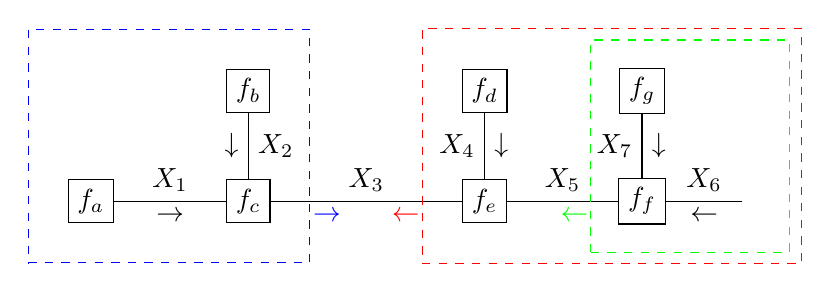
\begin{tikzpicture}[ node distance=20mm, auto, >=stealth ] 


% factors
\node (fa) [factor]						{$f_a$}; 
\node (fc) [factor,right of=fa]			{$f_c$};
\node (fb) [factor,short,above of=fc]	{$f_b$}; 
\node (fe) [factor,long,right of=fc]	{$f_e$}; 
\node (fd) [factor,short,above of=fe]	{$f_d$}; 
\node (ff) [factor,right of=fe]	{$f_f$};
\node (fg) [factor,short,above of=ff]	{$f_g$}; 
\node (fh) [terminal,short,right of=ff]	{};

% edges 
\path (fa) edge[-] 
  node[above] {$X_1$} 
  node[below] {$\rightarrow$} (fc);
\path (fb) edge[-] 
  node[right] {$X_2$} 
  node[left] {$\downarrow$} (fc);
\path (fc) edge[-] 
  node[above] {$X_3$} 
  node (m3) [below,blue,xshift=-.5cm] {$\rightarrow$} 
  node[below,red, xshift= .5cm] {$\leftarrow$} (fe);
\path (fd) edge[-] 
  node[left] {$X_4$} 
  node[right] {$\downarrow$} (fe);
\path (ff) edge[-] 
  node[above] {$X_5$} 
  node[below,green,xshift=.15cm] {$\leftarrow$} (fe);
\path (fg) edge[-] 
  node[left]  {$X_7$} 
  node[right] {$\downarrow$} (ff);
\path (fh) edge[-] 
  node[above] {$X_6$} 
  node[below] {$\leftarrow$} (ff);


% boxes 
\node (box_abc)   [box,dashed,blue,inner sep=5mm,fit=(fa)(fb)(fc)]        {};
\node (box_fgh)   [box,dashed,green,inner sep=3.5mm,fit=(ff)(fg)(fh)]       {};
\node (box_defgh) [box,dashed,red,inner sep=5mm,fit=(fd)(fe)(ff)(fg)(fh)] {};

 
% messages
%\draw[help lines] (0,0) grid (5,5);
%\draw [->, right of = box_abc >=stealth]; 

%\node[terminal] (fX1) { };
%
%\node[factor,right of=fA] (fB) {$f_B$} edge[-] node[below] {$X_3$} (fA); 
%\node[terminal,short,right of=fB] (fX5) {} edge[-] node[below] {$X_5$} (fB); 
%\node[terminal,short,below of=fA] (fX2) {} edge[-] node[left] {$X_2$} (fA); 
%\node[factor,short,below of=fB] (fC) {$f_C$} edge[-] node[left] {$X_4$} (fB); 



\end{tikzpicture}
\end{document}